\section{Zadanie 10}
Niech \(X, Y\) będą niezależnymi zmiennymi losowymi o rozkładzie \(N(0, 1)\). Wyznacz rozkład zmiennej losowej \(Z = \frac{X}{Y}\).

\subsection*{Rozwiązanie}

\begin{center}
	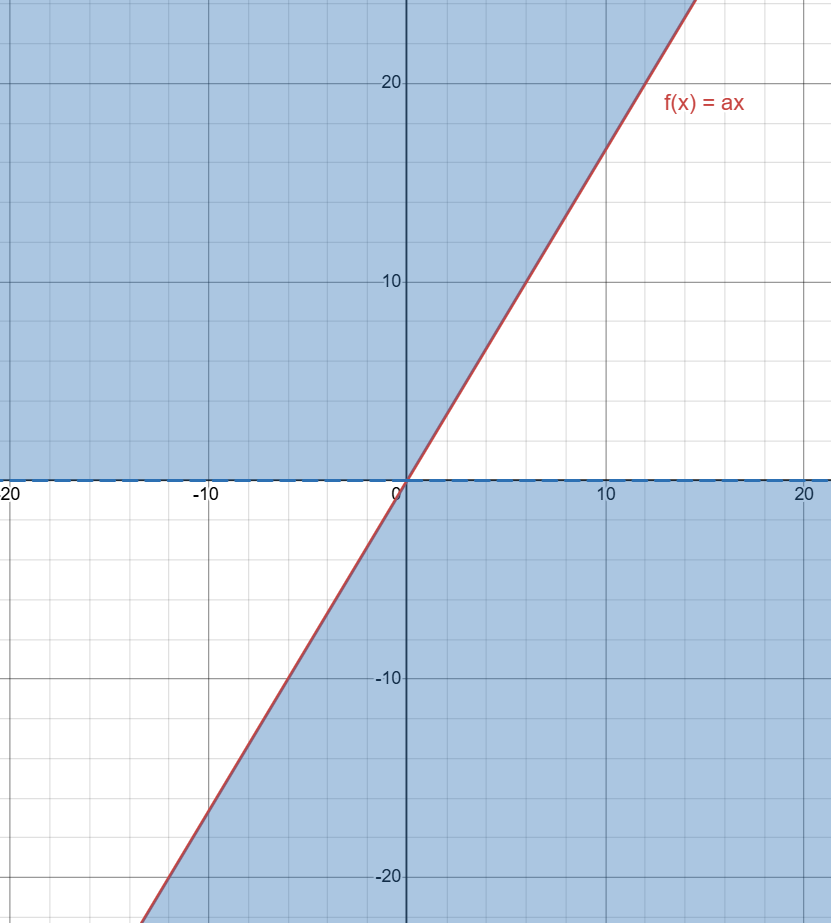
\includegraphics[width=0.45\textwidth]{tasks/10_obszar.png}
\end{center}

Policzymy dystrybuantę, całka musi być liczona po obszarze, który wyznacza wyrażenie
w prawdopodobieństwie (obszar zaznaczony na rysunku):

\[
	P\left(\frac{X}{Y} \le a \right)
\]

Nierówność
\[
	\frac{X}{Y} \le a
\]
jest równoważna
\[
	X \le aY \quad \text{dla } Y>0,
	\qquad
	X \ge aY \quad \text{dla } Y<0.
\]

Ponieważ zmienne losowe \(X\) i \(Y\) są niezależne oraz mają rozkład normalny
\(N(0,1)\), ich wspólna gęstość to iloczyn gęstości i ma postać:
\[
	f_{X,Y}(x,y)=\frac{1}{2\pi}e^{-\frac{x^2+y^2}{2}}.
\]

Dystrybuanta zmiennej \(\frac{X}{Y}\) wynosi więc
\[
	P\left(\frac{X}{Y} \le a\right)
	=
	\int_{0}^{\infty}\int_{-\infty}^{ay}
	\frac{1}{2\pi}e^{-\frac{x^2+y^2}{2}}\,dx\,dy
	+
	\int_{-\infty}^{0}\int_{ay}^{\infty}
	\frac{1}{2\pi}e^{-\frac{x^2+y^2}{2}}\,dx\,dy.
\]

Patrząc na rysunek można dojść do wniosku, że łatwiej przejść po obszarze za pomocą kąta i promienia, a nie współrzędnych kartezjańskich. Wprowadzamy więc współrzędne biegunowe:
\[
	x=r\cos\theta,\qquad y=r\sin\theta,
\]
Wówczas
\[
	x^2 + y^2 = r^2,
	\qquad
	dx\,dy = r\,dr\,d\theta,
\]
a gęstość wspólna przyjmuje postać
\[
	\frac{1}{2\pi} e^{-\frac{r^2}{2}} r\,dr\,d\theta.
\]

\[
	P\left(\frac{X}{Y} \le a\right)
	=
	\int_{0}^{\infty}\int_{\arctan{\frac{1}{a}}}^{\pi}
	\frac{1}{2\pi}e^{-\frac{r^2}{2}}r\,d\theta\,dr
	+
	\int_{0}^{\infty}\int_{\pi + \arctan\frac{1}{a}}^{2\pi}
	\frac{1}{2\pi}e^{-\frac{r^2}{2}}r\,d\theta\,dr.
\]
Wyciągając stałe przed całki otrzymujemy
\[
	P\left(\frac{X}{Y} \le a\right)
	=
	\frac{1}{2\pi}
	\left(
	\int_{0}^{\infty} e^{-\frac{r^2}{2}} r \, dr
	\right)
	\left(
	\int_{\arctan\frac{1}{a}}^{\pi} d\theta
	+
	\int_{\pi + \arctan\frac{1}{a}}^{2\pi} d\theta
	\right).
\]

Najpierw liczymy całkę po zmiennej \(r\):
\[
	\int_{0}^{\infty} e^{-\frac{r^2}{2}} r \, dr
	=
	\left[ -e^{-\frac{r^2}{2}} \right]_{0}^{\infty}
	=
	1.
\]

Teraz liczymy całki po kącie:
\[
	\int_{\arctan\frac{1}{a}}^{\pi} d\theta
	=
	\pi - \arctan\frac{1}{a},
\]
\[
	\int_{\pi + \arctan\frac{1}{a}}^{2\pi} d\theta
	=
	2\pi - \left(\pi + \arctan\frac{1}{a}\right)
	=
	\pi - \arctan\frac{1}{a}.
\]

Zatem
\[
	P\left(\frac{X}{Y} \le a\right)
	=
	\frac{1}{2\pi}
	\left(2\pi - 2\arctan\frac{1}{a}\right)
	=
	1 - \frac{1}{\pi}\arctan\frac{1}{a}.
\]
\[
	P\left(\frac{X}{Y} \le a\right)
	=
	1 - \frac{1}{\pi}\arctan\frac{1}{a} = 1-\frac{1}{\pi} \left(\frac{\pi}{2} -  \arctan{a} \right) = \frac{1}{2} + \frac{1}{\pi}\arctan{a} .
\]
Jest to dystrybuanta rozkładu Cauchy'ego

\subsection*{Odpowiedź}
\[
	\boxed{\frac{X}{Y} \sim Cauchy (0,1)}
\]
